\subsection*{Problema 20}

\textbf{Enunciado:} \\
Calcular la integral indefinida:
\begin{align*}
\int \dfrac{\cos^3 x \, dx}{2 - \sin x}
\end{align*}

\textbf{Solución:} \\
Siguiendo la sugerencia, reescribimos el numerador utilizando la identidad pitagórica $\cos^2 x = 1 - \sin^2 x$:
\begin{align*}
\cos^3 x \, dx &= \cos^2 x \cdot \cos x \, dx \\
&= (1 - \sin^2 x)\cos x \, dx
\end{align*}

Sustituimos esto en la integral original:
\begin{align*}
I = \int \dfrac{(1 - \sin^2 x)\cos x}{2 - \sin x} \, dx
\end{align*}

Realizamos el cambio de variable propuesto:
\begin{align*}
u &= \sin x \\
du &= \cos x \, dx
\end{align*}

Sustituyendo $u$ y $du$ en la integral, obtenemos una función racional:
\begin{align*}
I = \int \dfrac{1 - u^2}{2 - u} \, du
\end{align*}

Para integrar esta función racional, realizamos la división polinómica o reescribimos el numerador. Notemos que $1 - u^2 = (1 - u)(1 + u) = -(u - 1)(u + 1)$. Dividiendo $u^2 - 1$ entre $u - 2$:
\begin{align*}
\dfrac{u^2 - 1}{u - 2} = u + 2 + \dfrac{3}{u - 2}
\end{align*}

Por lo tanto, la integral se descompone en términos más simples:
\begin{align*}
I &= \int \left( u + 2 + \dfrac{3}{u - 2} \right) du
\end{align*}

Integramos cada término de manera directa:
\begin{align*}
I = \dfrac{u^2}{2} + 2u + 3\ln|u - 2| + C
\end{align*}

Finalmente, regresamos a la variable original $x$ sustituyendo $u = \sin x$:
\begin{align*}
I = &\dfrac{\sin^2 x}{2} + 2\sin x \\
&+ 3\ln|\sin x - 2| + C
\end{align*}

Como $\sin x \le 1$ para todo número real $x$, el argumento del valor absoluto $(\sin x - 2)$ es siempre negativo. Por ende, podemos expresar el resultado final como:
\begin{align*}
\int &\dfrac{\cos^3 x \, dx}{2 - \sin x} = \dfrac{1}{2}\sin^2 x \\
&+ 2\sin x + 3\ln(2 - \sin x) + C
\end{align*}

\begin{figure}[H]
	\centering
	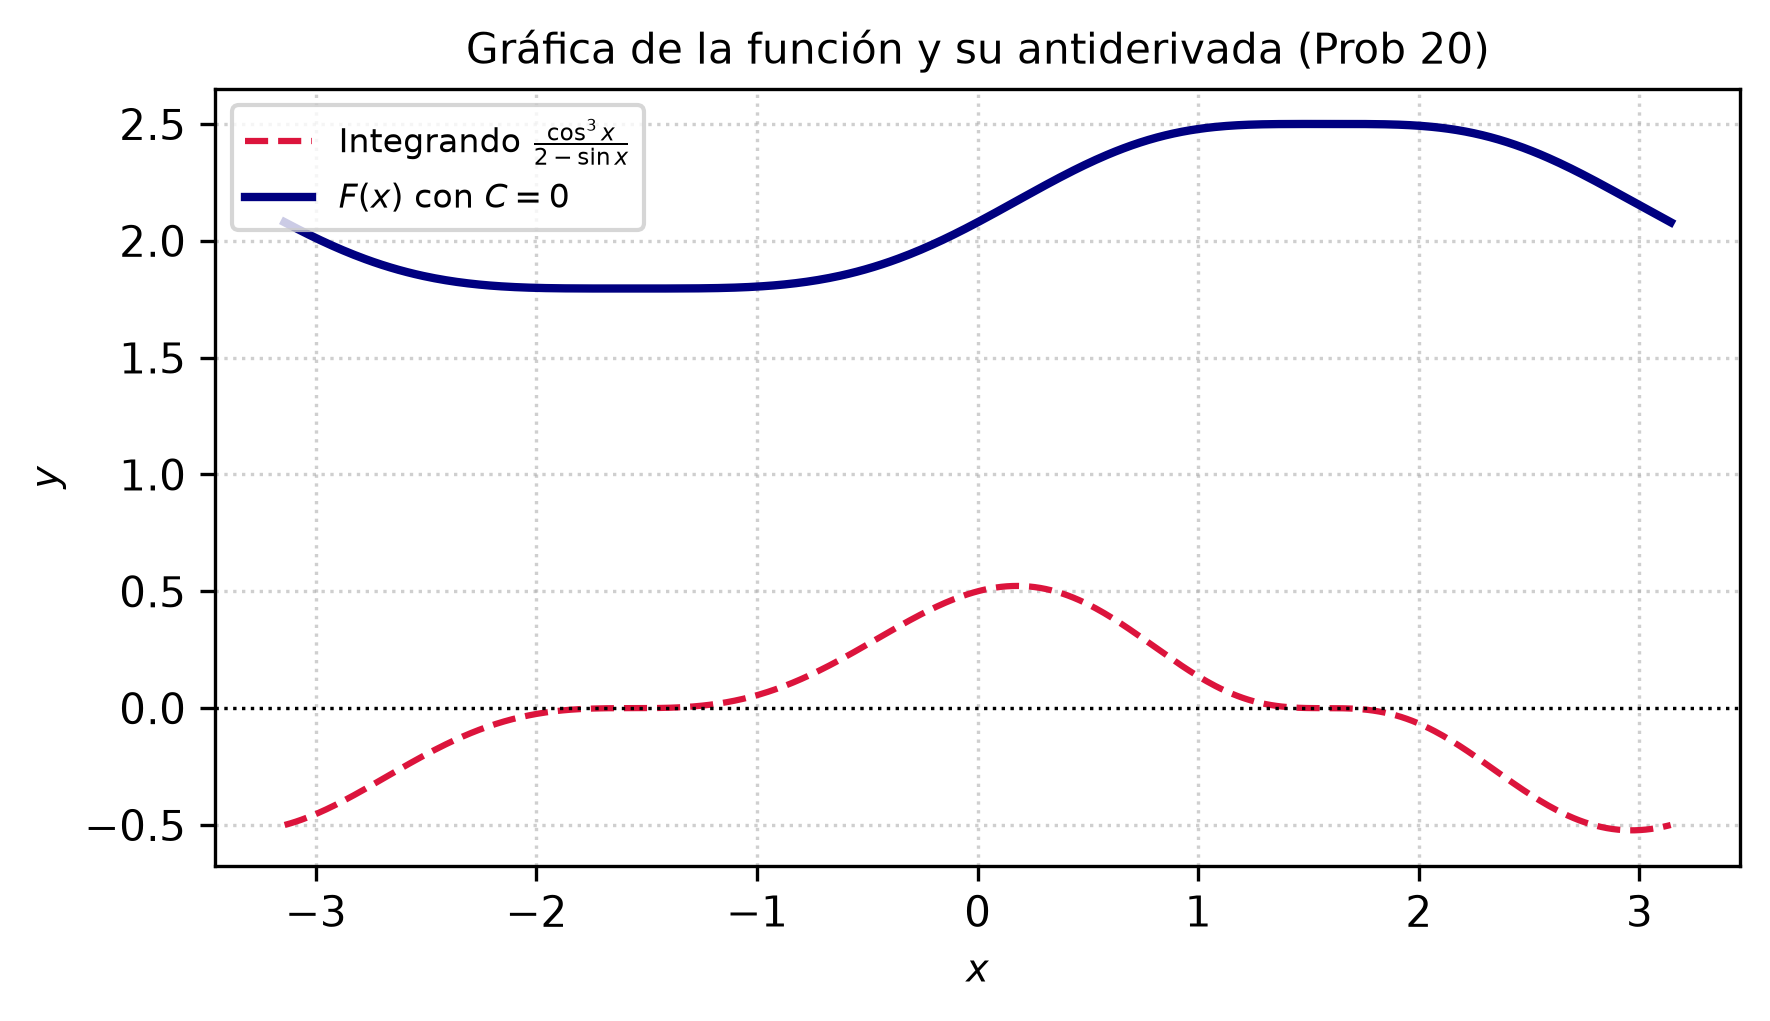
\includegraphics[width=\columnwidth]{semana_04/graficas/SEM04_P20_grafica.png}
	\caption{Representación gráfica de $f(x)$ y su antiderivada $F(x)$ evaluada para la constante de integración $C = 0$ (Problema 20).}
	\label{fig:problema20}
\end{figure}
